\documentclass[a4paper,12pt]{report}
\usepackage[T2A]{fontenc}
\usepackage[utf8]{inputenc}
\usepackage[english,russian]{babel}
\usepackage{circuitikz}
\usepackage{wrapfig}
\usepackage{makecell}
\usepackage{tabularx}
\usepackage{graphicx}
\usepackage{gensymb}
\usepackage{cancel} %cancel symbol
\usepackage{amsmath,amsfonts,amssymb,amsthm,mathtools}
\usepackage{pgfplots}
%\usepackage[margin=3cm]{geometry}
\pgfplotsset{compat=1.12}
\usepackage{mathrsfs}

%tikz (draw)

\usepackage{tikz}
\usepackage{pstricks-add}
%tikz libraries

\usetikzlibrary{intersections}
\usetikzlibrary{arrows.meta}
\usetikzlibrary{calc,angles,positioning}
\usetikzlibrary{arrows}
\usepackage{float}

\parindent=0ex
\setlength{\parskip}{\baselineskip}%
\setlength{\parindent}{0pt}%

\graphicspath{ {C:/Users/George/Documents/MIPT_TEX/} }

\newcommand{\R}{{\mathbb R}}
\newcommand{\N}{{\mathbb N}}
\newcommand{\fancy}[1]{{\mathbb{#1}}}
\DeclareMathOperator{\sgn}{sgn}
\newtheorem{problem}{Задача}[]
\newenvironment{sol}{\paragraph{Решение}}{}
\renewcommand\thesection{\arabic{section}}
\newcommand{\uni}{\cup}
\newcommand{\inter}{\cap}

\begin{document}
	

\begin{titlepage}
	\begin{center}
		МОСКОВСКИЙ ФИЗИКО-ТЕХНИЧЕСКИЙ ИНСТИТУТ (НАЦИОНАЛЬНЫЙ ИССЛЕДОВАТЕЛЬСКИЙ УНИВЕРСИТЕТ) \\
		
		
		\hfill \break
		Факультет обшей и прикладной физики\\
		\vspace{2.5cm}
		\large{\textbf{Отчёт по лабораторной работе 1.2.5 <<Исследование прецессии уравновешенного гороскопа>>}}\\
		\hfill \break
		\\
	\end{center}
	
	\begin{flushright}
		Выполнил:\\
		Студент гр. Б02-304\\
		Головинов. Г.А.
	\end{flushright}
	
	\vspace{7cm}
	
	\begin{center}
		
\includegraphics[width=0.15\linewidth]{uni}
	\end{center}
	

	

	\vfill
	
	\begin{center} Долгопрудный, 2023 \end{center}
	
	\thispagestyle{empty}
	
\end{titlepage}


	\newpage
	\pagenumbering{arabic}
    
    \subsection*{Аннотация}
        \paragraph*{Цель работы:} измерить коэффициент теплопроводности воздуха при атмосферном давлении в зависимости от температуры.
        \paragraph*{В работе используются:} цилиндрическая колба с натянутой по оси нитью, термостат, вольтметр и амперметр, источник постоянного напряжения, магазин сопротивлений.
    \subsection*{Основные теоретические сведения}
    Теплопроводность -- процесс передачи тепловой энергии от нагретых частей системы к холодным за счет хаотического движения частиц среды. В газах теплопроводность осуществляется за счет непосредственной передачи кинетической энергии от быстрых молекул к медленным. Перенос тепла описывается законом Фурье.
    \paragraph*{Закон Фурье}
    Этот закон утверждает, что плотность потока энергии $\vec{q}$ (количество теплоты, переносимое через единичную площадку за единицу времени) пропорциональна градиенту температуры $\nabla T$:
    \begin{equation}
        \label{fourier}
        \vec{q}=-\kappa \nabla T
    \end{equation}
    где $\kappa$ -- коэффициент теплопроводности. [$\kappa$]=$\frac{\text{Вт}}{\text{м}\cdot\text{К}}$

    Молекулярно-кинетическая теория дает оценку коэффициента теплопроводности газов:
    \begin{equation}
        \label{kappa approx}
        \kappa \sim \lambda \vec{v} \cdot n C_V
    \end{equation}
    здесь $\lambda$ -- длина свободного пробега молекул газа, $\vec{v}=\sqrt{\frac{8kT}{\pi m}}$ -- средняя скорость теплового движения, $n$ -- концентрация молекул, $C_V=\frac{i}{2}k$ -- теплоемкость при постоянном объеме в расчете на одну молекулу

    Формула \eqref{kappa approx} дает лишь оценку по порядку величины, а также правильную функциональную зависимость. Коэффициент перед этой формулой зависит от закона взаимодействия молекул и не может быть вычислено методами общей физики. Также не подлежит прямому измерению длина свободного пробега.

    Ее можно оценить как $\lambda=1/n\sigma$, где $\sigma$ -- эффективное сечение столкновения молекул друг с другом -- величина, характеризующая вероятность существенного отклонения налетающей частицы при взаимодействии с некоторым рассеивающим центром. В общем случае определяется как отношение плотности потока рассеянных частиц к плотности потока падающих, имеет размерность площади.

    В простейшей модели $\sigma=const$, а коэффициент теплопроводности пропорционален корню абсолютной температуры: $\kappa\sim\vec{v}/\sigma\sim\sqrt{T}$. На практике сечение $\sigma$ зависит от температуры и его следует считать медленно убывающей функцией.

    Рассмотрим теплопроводность в цилиндрической геометрии:
    \begin{wrapfigure}{R}{0.3\textwidth}
        \vspace{-5mm}
        \centering
        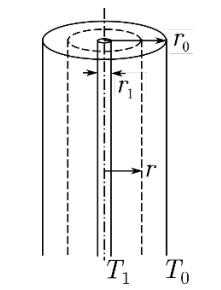
\includegraphics[width=0.7\linewidth]{img/geometry}
        \caption{Геометрия установки}
    \end{wrapfigure}

    Пусть тонкая нить радиусом $r_1$ и длиной $L$ помещена на оси цилиндра радиуса $r_0$. Температура стенок $T_0$ поддерживается постоянной. Пусть в нити выделяется некоторая тепловая мощность $Q$ [Вт]. Если цилиндр длинный ($L\gg r_0$), то можно пренебречь теплоотводом через его торцы. Тогда все параметры газа можно считать зависящими только от расстояния $r$ до оси цилиндра, а поток $\vec{q}$ -- направленным строго радиально (от оси).

    Вместо уравнения \eqref{fourier} имеем теперь:
    \begin{equation}
        \label{q new}
        q=-\kappa\frac{dT}{dr}
    \end{equation}
    В стационарном состоянии полный поток тепла через цилиндрическую поверхность радиуса $r$ и площадью $S=2\pi rL$ должен быть одинаков и равен $Q=qS$:
    \begin{equation}
        \label{Q}
        Q=-2\pi r L\cdot \kappa \frac{dT}{dr}=const
    \end{equation}
    Считая перепад температуры сильно меньшим чем само значение температуры ($\Delta \ll T_0$) можно пренебречь изменением теплопроводности $\kappa$ от радиуса. Тогда можно проинтегрировать по радиусу и температуре:
    \begin{equation*}
        Q\int_{r_1}^{r_0}\frac{dr}{r}=-2\pi L\cdot \kappa  \int_{T_1}^{T_0}dT 
    \end{equation*}
    \begin{equation*}
        Q\ln(r_0/r_1)=2\pi L \cdot \kappa \Delta T, \quad \Delta T=T_1-T_0
    \end{equation*}
    \begin{equation}
        \label{Qfinal}
        Q=\frac{2\pi L\kappa\Delta T}{\ln (r_0/r_1)}
    \end{equation}

    \paragraph*{Оценка времени установления равновесия} Когда в процессе работы мы меняем (желаемую) температуру на термостате требуется некоторое время, чтобы жидкость достигла этой температуры, затем некоторое время, чтобы жидкость достигла стенок цилиндра, затем некоторое время, чтобы воздух в цилиндре тоже прогрелся до новой температуры. Оценим время установления нового состояния в системе (без учета нагрева термостата).

    Рассмотрим плоский слой толщиной $a$ и сечением $S$, заполненный газом при постоянном давлении. Пусть температура одной из граней выросла на некоторую $\Delta T$. Это вызовет поток тепла в сторону более холодной грани, величину которого можно оценить по закону Фурье: $q\sim \kappa \Delta T/a$. Для того чтобы весь слой прогрелся на $\Delta T$ в него должно поступить тепло $nSa\cdot C_p\Delta T$, где $C_p$ -- теплоемкость при постоянном давлении в расчете на одну молекулу.

    С другой стороны, поступившее за это время $\tau$ тепло можно вычислить как $qS\tau=\kappa\frac{\Delta T}{a}S\tau$. Приравнивая находим:
    \begin{equation*}
        nSaC_p\Delta T=\kappa\frac{\Delta T}{a}S\tau
    \end{equation*}
    тогда
    \begin{equation}
        \label{tau}
        \tau\sim\frac{C_pa^2n}{\kappa}
    \end{equation}
    Коэффициент $\chi=\frac{\kappa}{C_pn}$ называется температуропроводностью среды. Для воздуха при нормальных условиях $\chi\sim 0.2cm^2/s$, что при размере $a\sim 1cm$ имеет характерное время $\tau\sim 5s$

    Таким образом, состояние в установке может устанавливаться в течение нескольких десятков секунд, поэтому, учитывая также прогрев трубок, стоит ждать несколько минут после достижения термостатом желаемой температуры.

    \paragraph*{Пределы применимости теории} Закон Фурье может нарушаться, когда масштабы установки соизмеримы с длиной свободного пробега молекул. Это может привести к эффекту, известному как <<температурный скачок>>, явление, когда температура нити может отличаться от температуры окружающего газа. В данной работе этим можно пренебречь, так как при нормальных условиях $\lambda\sim 10^{-5}cm$, что сильно меньше размеров системы, и даже размеров нити.

    Также возможны другие механизмы теплопередачи: конвекция и излучение. Конвекция возникает в поле тяжести только при больших вертикальных градиентах температуры, поэтому установка расположена вертикально. Мощность излучения можно оценить по закону\newline Стефана-Больцмана:
    \begin{equation}
        \label{stef-bolz}
        Q_{rad}=\epsilon S \sigma_S(T_1^4-T_0^4)\approx 4\epsilon S\sigma_ST_0^3\Delta T
    \end{equation}
    где $S$ -- площадь поверхности нити, $\sigma_S=5.67\cdot 10^{-8}W/(m^2K^4)$ -- постоянная Стефана-Больцмана, $\epsilon$ -- безразмерный <<коэффициент черноты>>, зависящий от качества и материала излучающей поверхности. Для металлов с полированной поверхностью можно принять $\epsilon\sim 0.1-0.2$. По формуле \eqref{stef-bolz} находим мощность излучения:
    \begin{equation*}
        Q_{max} \approx 3mW
    \end{equation*}

    \subsection*{Экспериментальная установка}
    \begin{wrapfigure}{R}{0.5\textwidth}
        \vspace{0mm}
        \centering
        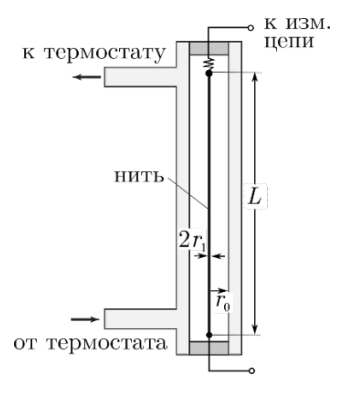
\includegraphics[width=0.7\linewidth]{img/ustanovka}
    \end{wrapfigure}

    Установка представляет собой цилиндрическую трубку длиной $L=40cm$, диаметром $2r_0=1cm$, диаметр нити $2r_1=50\mu m$. Трубка заполнена воздухом, через небольшое отверстие воздух внутри системы может сообщаться с атмосферой. Стенки трубки помещены в кожух, через который пропускается вода из термостата, так что температура стенок $T_0$ поддерживается постоянной. Трубка расположена вертикально для предотвращения влияния конвекции, как было обговорено ранее.

    Нить служит источником тепла:
    \begin{equation}
        \label{q wire}
        Q=UI
    \end{equation}
    где Q -- мощность нагрева нити, U -- напряжение на нити, I -- сила тока.
    
    Также нить является способом измерения температуры.  Сопротивление нити можно найти по закону Ома:
    \begin{equation}
        \label{ohm}
        R=\frac{U}{I}
    \end{equation}  
    
    Электрические приборы и нить подключены согласно следующей схеме:

    \begin{figure}[H]
    \centering
    \begin{circuitikz}[>=latex', european, scale=1.3]
    \tikzstyle{block} = [draw, rectangle, minimum height=1cm, minimum width=2cm]
    \draw (2.0,-0.0) to[R,l=$R$] (4.0,-0.0);
    \draw (0.0,-0.0) to[battery1,l=$\varepsilon$, invert] (2.0,-0.0);
    \draw (4.0,-0.0) to[R,l=$R_\text{н}$] (4.0,-3.5);
    \draw (4.0,-0.0) to[short] (5.5,-0.0);
    \draw (5.5,-0.0) to[rmeter, t=$U$] (5.5,-3.5);
    \draw (5.5,-3.5) to[short] (0.0,-3.5);
    \draw (0.0,-3.5) to[rmeter, t=$I$] (0.0,-0.0);
    \end{circuitikz}
    \caption{Схема цепи}
    \end{figure}

    Предполагая, что все компоненты цепи идеальны, измерив напряжение $U$ и силу тока $I$ можно найти мощность, выделяемую на нити и ее сопротивление. По этим данным мы будем строить зависимость $R(Q)$ -- нагрузочная кривая.

    Уменьшая сопротивление магазина мы увеличиваем значение силы тока в цепи. Есть некоторое значение силы тока $I_{max}$, выше которой теплопроводности воздуха перестанет хватать, чтобы отводить тепло, выделяющееся на нити. Если это значение превысить, нить может перегореть.

    Найдем максимальную мощность отвода воздуха по формуле \eqref{Qfinal}, затем используя формулу $Q_{w}=I^2 R$, считая $R\approx 20 \Omega$ получим, что $I_{max}\approx 137 mA$, если максимальная разница температур $\Delta T\approx 20 K$

    Зависимость $R(T)$ -- сопротивления от температуры при температурах около комнатной (0-100$C^\circ$) можно с достаточно большой точностью считать линейной зависимостью:
    \begin{equation*}
        R(T)\approx R_0+\alpha(T-T_0)
    \end{equation*}
    гда $\alpha$ -- коэффициент пропорциональности, $R_0$ -- сопротивление при температуре $T_0$.
    Мы в ходе работы также проверим ее линейность.
    
\end{document}